\documentclass[conference]{IEEEtran}
\usepackage{times}

% numbers option provides compact numerical references in the text. 
\usepackage[numbers]{natbib}
\usepackage{multicol}
\usepackage[bookmarks=true]{hyperref}
\usepackage{graphics} % for pdf, bitmapped graphics files
\usepackage{graphicx}
\usepackage{amsmath,amssymb,latexsym,float,epsfig,subfigure}
\usepackage{amsmath} % assumes amsmath package installed
\usepackage{amssymb}  % assumes amsmath package installed
\usepackage{lipsum}
\usepackage[export]{adjustbox}
\usepackage[normalem]{ulem} % underline
\usepackage{wrapfig}
\usepackage{multirow}
\usepackage{balance}
\usepackage{color}
\usepackage{url}
\newcommand{\argmax}{\arg\!\max}
\newcommand{\norm}[1]{\left\lVert#1\right\rVert}
\pdfinfo{
   /Author (Homer Simpson)
   /Title  (Robots: Our new overlords)
   /CreationDate (D:20101201120000)
   /Subject (Robots)
   /Keywords (Robots;Overlords)
}

\begin{document}

% paper title
\title{Mode switch assistance maximizing confidence disambiguation}

% You will get a Paper-ID when submitting a pdf file to the conference system
%\author{Deepak Gopinath and Brenna D. Argall}

\author{\authorblockN{Deepak Gopinath}
\authorblockA{Department of Mechanical\\Engineering,
Northwestern University\\
Evanston, Illinois 30332\\
Email: deepakedakkattilgopinath2015\\@u.northwestern.edu}
\and
\authorblockN{Brenna D. Argall}
\authorblockA{Department of Mechanical\\Engineering,
		Northwestern University\\
		Evanston, Illinois 30332\\
		Email: brenna.argall@northwestern.edu}}


% avoiding spaces at the end of the author lines is not a problem with
% conference papers because we don't use \thanks or \IEEEmembership


% for over three affiliations, or if they all won't fit within the width
% of the page, use this alternative format:
% 
%\author{\authorblockN{Michael Shell\authorrefmark{1},
%Homer Simpson\authorrefmark{2},
%James Kirk\authorrefmark{3}, 
%Montgomery Scott\authorrefmark{3} and
%Eldon Tyrell\authorrefmark{4}}
%\authorblockA{\authorrefmark{1}School of Electrical and Computer Engineering\\
%Georgia Institute of Technology,
%Atlanta, Georgia 30332--0250\\ Email: mshell@ece.gatech.edu}
%\authorblockA{\authorrefmark{2}Twentieth Century Fox, Springfield, USA\\
%Email: homer@thesimpsons.com}
%\authorblockA{\authorrefmark{3}Starfleet Academy, San Francisco, California 96678-2391\\
%Telephone: (800) 555--1212, Fax: (888) 555--1212}
%\authorblockA{\authorrefmark{4}Tyrell Inc., 123 Replicant Street, Los Angeles, California 90210--4321}}


\maketitle

\begin{abstract}
The abstract goes here.
\end{abstract}

\IEEEpeerreviewmaketitle

\section{Introduction}

Assistive and rehabilitation devices such as powered wheelchairs, robotic arms and myoelectric prosthesis play an important role in the lives of people with motor impairments. These devices help to increase their ability to perform activities of daily lives and reduce their dependence on caretakers and is crucial to revolutionizing the way they interact with society. As the field of assistive robotics progresses rapidly, the devices themselves have become more capable and dextrous and as a result more complex, high dimensional and harder to control. 

A possible paradigm for control of such high dimensional devices is one in which the human is a \textit{provider of motion}. The confounding factor is that the more severe a person's motor impairment, the more limited are the control interfaces available to them to operate. These interfaces (for example, head arrays and Sip-N-puffs) are lower in dimensionality and bandwidth and usually requires more number of mode switches for successful task completion. Thus, a greater need for sophisticated assistive devices is paired with a diminishing ability to control their additional complexity. 

Due to the dimensionality mismatch between the control interface and the robotic device, control interfaces can only operate in \textit{modes} which correspond to differents parts of the control space. More limited the control interface is, more the number of modes there are. In order to have full control of the robot (6D for an assistive robotic arm) the user will have to switch between the difference partitions of the control space and this is known as \textit{mode switching}. 

It has been established that mode switching is expensive and as a result task performance is degraded. Furthermore, it adds to the cognitive and physical burden as each of these mode switches will require the user to shift their attention from the task to performing the mode switch. The introduction of shared autonomy to these systems helps to alleviate and address some of these issues by letting the system take responsibility to some extent, thereby reducing the human effort in achieving a goal. 

Shared autonomy paradigms in assistive robotics can be broadly classified into two categories: \textit{heirarchical} and \textit{blending}. An example of a \textit{hierarchical} assistance system is one in which the user acts as an indicator of the goal and the robot executes the motion autonomously. In a \textit{blending} based assistance paradigm, the robot and the human work in the same control space (for example, velocity blending in Cartesian space) and usually the final control command issued to the robot is a blended sum of an autonomous robot policy and the control command issued by the human. 
\begin{figure}[t]
	\centering
	\includegraphics[width = 0.8\hsize]{./figures/DE.png}
	\caption{}
	\label{DE}
\end{figure}
In this paper, we develop a mode switching assistance paradigm that augments a blending based shared control system for an assistive robotic arm. For the underlying blending based shared control, the assistance provided by the robot is regulated by the robot's ability to estimate user intent confidently and accurately and it is very unlikely that the robot will be able to determine this with a 100\% accuracy.  Therefore the blending factor is usually a function of a confidence metric. This confidence metric is the system's confidence in its own estimate of human intent and is usually a function of the human control command, the autonomous policy, robot pose, goal locations \textit{et cetera}. This implies that human control actions have a direct impact on the confidence measure. 


However, it can be the case that certain actions by the human (the only way to issue actions are through the control interface) or equivalently certain control commands issued by the humans might carry more information and better expresses the human intent which can then help the robot to draw useful and correct inferences about intent more easily. That is certain human actions are more \textit{legible} than others. A \textit{legible} motion in this context is one which will help the observer (or the system) decipher the intent behind the action more \textit{quickly} and \textit{confidently}. However, the control commands that a human can generate is limited by the control mode in which he/she is operating.

Consider the example illustrated in Figure~\ref{DE}. In this 2D world, A and B indicate two point goal locations. The robot end effector is at location C. It is clear that any motion of the end effector along the y-axis will not help the system disambiguate between the two goals; that is the motion is not legible. However, if the human moves the robot along the x-axis, the system will be able to infer the goal immediately based on the direction in which the robot moves. That is, in this example, a human control command issued along the $x$ dimension is more \textit{intent expressive} and helps the robot to provide the right kind of assistance more quickly and confidently. 

With the mode switching assistance scheme developed in this work, we hope to elicit more legible human control commands by placing the user control in those modes that will have \textit{maximal confidence disambiguation} between the various goals in the scene. 

Furthermore, the commonplace notion in human-robot interaction and especially in assistive robotics is that ``help'' is provided solely by the robot. In addition to eliciting more legible motion from the human, we also seek to explore and exploit the underlying synergies in human robot interaction to facilitate more seamless and efficient task execution. The idea of ``people helping robots helping people'' is key to this work and by requiring the human to operate in a mode that will potentially help the robot in deciphering the human's intent more confidently, the human, in some sense, helps the robot so that it provide ``help'' in the most effective manner. 
It is possible that in some cases such a mode might not be the most ideal mode \textit{for} the human to operate in due to personal preferences. However, if the human agrees to compromise a little bit and provides ``hints" and ``nudges" the robot in the right direction, the overall performance gain will likely outweigh the slight sub-optimality due to the ``wrong'' mode. 

In Section \ref{RW} we present an overview of the relevant research in the area of shared control in assistance systems focusing on mode switching, legibility of motion and synergies in human robot interaction. Section \ref{ALGO} describes the mathematical formalism for the algorithm and the metric used for confidence disambiguation. The study methods, tasks and metrics are discussed in Section \ref{EXP}. In Section \ref{RES} we present the preliminary results from our pilot study and discussions followed by conclusions in Section \ref{CON}

\section{RELATED WORKS}\label{RW} 

Shared control assistance paradigms help to offload cognitive and physical burden~\cite{volosyak2005rehabilitation} without requiring the user to relinquish complete control and is usually preferred over fully autonomous assistive robotic systems for reasons of both robustness and user satisfaction. One possible way to control high dimensional assistive devices such as robotic arms is to partition the control space (6D for a robotic arm) into subsets called \textit{modes} and have the user control one mode at a time using control interfaces such as joysticks~\cite{tsui2008development}, head arrays and sip-and-puffs. This is known as \textit{modal control}.

Herlant et al. assesses the difficulties faced by users when they operate these devices using \textit{modal control} in \cite{herlant2016assistive}. In their work they report that a significant number of users found \textit{mode switching} to be slow and burdensome. The cognitive burden of shifting focus (also known as \textit{task switching})  from the task at hand to mode switches can result in a significant decrease in task performance regardless of the control modality~\cite{monsell2003task}. 

\citet{herlant2016assistive} also proposes a time-optimal mode switch assistance paradigm and evaluates the performance of the same in a simulated 2D robot and provides insight into the fact that even a simple time optimal automatic mode switching system can significantly improve user satisfaction while maintaining the quality task performance. However, our present system is not motivated by ad hoc assumptions regarding the optimizing principles at work when a user operates a robot. In a previous study~\cite{gopinath2017human} that we conducted, we found that it is not always the case that users are trying to optimize for time or effort during task execution. 

Our present system is intended to bring out an intent-expressive control command that is more legible from the human, so that the system is able to infer the correct goal more quickly and confidently. Legibility and predictability of robot motion has been thoroughly investigated and different methods for generating legible robot motion have been proposed by Dragan et al. in \cite{dragan2013legibility,dragan2013generating}. Unlike their work in which the primary concern was to make robot's motion more legible to the human observer, in this paper we deploy similar concepts of legibility to the human control commands such the intent expressed in the command is clear \textit{to} the robot. In most cases the human knows beforehand what goal he/she is going for and therefore the motion generated by the human is usually \textit{predictable}. As long as the confidence measure used in the underlying blending paradigm captures the predictable aspect of human generated robot motion, the mode switching assistance proposed by us will place user control in that mode which can provide maximal confidence disambiguation thereby improving the legibility.

Our assistance system also seeks to enhance mutual cooperation and the underlying synergies that are crucial for successful human-robot interaction. Sorokin et al. proposes a framework in which for human-robot interaction in which humans provide semantic information and judgments about the environment to the robot which then utilizes them to improves its own capabilities~\cite{sorokin2010people}. Rosenthal et al. proposes a \textit{symbiotic} human robot interaction scheme which aims to overcome perceptual and cognitive limitations that robots might encounter while still allowing the robots to help humans as well~\cite{rosenthal2010effective}. 



%2-4 works which investigates what legibility means, proposes ways to generate legible robot motion. In all these works, the goal is to make the motion more legible for the human. In our system, we want the human to move the robot in a way that the intent is more legible FOR the system. That is the roles are reversed. Since the human knows beforehand what goal he/she is going after the motion generated by the human is usually predictable. As long as the confidence measure is able to capitalize on this predictability, the system can force the human to generate legible motions by requiring them to operate in those modes which can provide maximal confidence disambiguation. The notion of a confidence mediated blending paradigm is formalized in other Dragan paper. 
%
%Discuss works which formalizes legibility. Talk about how in the present work we are flipping roles and concerned more about the legibility of human's actions (which causes robot motion). Dragan et al. formalizes and investigates legibility and predictability of robot motion. Their paper's concern was primarily to make a robot's motion more legible for the human who will the observer. In the present work, we use the principle of legibility, except that the robot and the human switch roles. The human controls the robot motion via a control interface and robot is the ``observer'' and the system seeks to elicit to legible indicators \textit{from} the human in order to provide more effective assistance.

%Discuss works which emphasize two way interaction for more gain. Look into this a little more closely. Synergy related work. 
%\begin{figure*}[t]
%	\centering
%	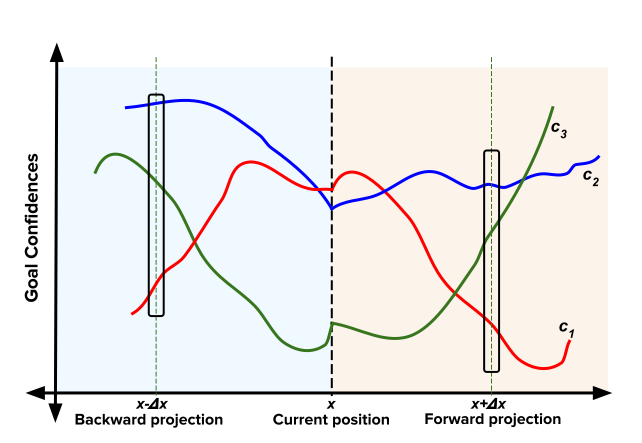
\includegraphics[width = 1\hsize, height = 0.45\vsize]{./figures/DisambMetric.jpg}
%	\caption{}
%	\label{DM}
%\end{figure*}
\section{ALGORITHM DESIGN} \label{ALGO}
This section describes the algorithm that is used to compute the control mode with maximal confidence disambiguation, thereby eliciting the most legible control command from the human. The details of the underlying blending based shared control system is also described briefly in this section.

\subsection{Notation}

%Let $g_i \in \mathcal{G} \;\; \forall \;\;i \in [1,2,\dots,n_g]$, denote the $n_g$ number of possible goals in the scene and $c_i \in \mathcal{C} \;\; \forall \;\;i \in [1,2,\dots,n_g]$ denote the confidence that the system has in each one of the $n_g$ goals.

Let $\mathcal{G}$ be the set of all candidate goals in the scene with $\vert\mathcal{G}\vert = n_g$ and let $g^{i}$ refer to the $i^{th}$ goal where $i \in [1,2,\dots,n_g]$. The set of goals result in an associated set of confidences which will be denoted as $\mathcal{C}$ and $c^{i}$ will refer to the confidence associated with goal $g^{i}$. Let $\mathcal{K}$ be the control space in which the robot operates ($\vert\mathcal{K}\vert = n_k$) and $k^{j}$ refer to an individual control dimension where $j \in [1,2,\dots,n_k]$.  The cardinality of $\mathcal{K}$ depends on the robotic platform, for example, in the case of a smart wheelchair $n_k = 2$ (heading and forward velocity) whereas for a 6 DOF robotic arm $n_k = 6$.
%Let $\mathcal{G}$ be the set of all candidate goals in the scene with $\vert\mathcal{G}\vert = n_g$, resulting in an associated distribution of confidences $c_g \in \mathcal{C} \;\;( \forall \; g \in \mathcal{G})$  over candidate goals. Let $\mathcal{K}$ be the control space in which the robot operates with $\vert\mathcal{K}\vert = n_k$.


For control purposes, the set $\mathcal{K}$ is partitioned into subsets known as \textit{modes}. Let $\mathcal{M}$ refer to the set of all modes that the control space $\mathcal{K}$ is partitioned into. The number of modes ($n_{cm}$) is specific to the control interface and mapping. Furthermore, let $m^{p}$ refer to the $p^{th}$ mode where $p \in [1,2,\dots,n_{cm}]$.
Another quantity of interest is the gradient of individual goal confidences along the separate control dimensions. More specifically, $\frac{\partial c^i}{\partial k^j}$ captures the rate of change of the $c^{i}$ along control dimension $k^{j}$. Furthermore, since the confidence function, in general, can assume drastically different values upon moving in positive and negative directions along a control dimension, the left and right gradients are explicitly denoted as $\frac{\partial c^i}{\partial k^j}^{+}$ and $\frac{\partial c^i}{\partial k^j}^{-}$ respectively. The specific form of the confidence function used in our study will be discussed in (denote section number), but the formalism developed in (refer to disambiguation metric section) is agnostic to a particular form of confidence function. Additionally, an analytical closed form expression for the gradient might not always be available as the confidence functions need not be continuous and differentiable. In other cases, due to the complexity of the confidence such an expression might be incredibly hard to compute. Therefore in our work, we numerically approximate the gradient by forward and backward differencing. 
%Lastly, we define a \textit{disambiguation} metric $D_{k_j}\in \mathbb{R}\; \forall \;k_j \in \mathcal{K}$ and is a function of the individual goal confidences $c_i$ and $\frac{\partial c_i}{\partial k_j}$\footnote{For the rest of the paper $\frac{\partial c_i}{\partial k_j}$ will be denoted as $ \dot{c}_{ij}$}. 
Lastly, we define a \textit{disambiguation} metric  $D_{k^j}\in \mathbb{R}\; \forall \;k^j \in \mathcal{K}$ and is a function of $c^i$ and $\frac{\partial c^i}{\partial k^j}$\footnote{For the rest of the paper $\frac{\partial c^i}{\partial k^j}$ will be denoted as $ \dot{c}^{i}_j$}. Similar to the gradients we explicitly define disambiguation metrics for both positive and negative directions as $D_{k_j}^{+}$ and $D_{k_j}^{-}$ respectively.

We also define a disambiguation metric $D_m \in \mathbb{R}$ for each control mode $m \in \mathcal{M}$.
The disambiguation metric $D_m$ is a measure of how legible the robot motion will be if the user were to control the robot in mode $m$. The higher the value, the easier it will be for the system to infer the human intent. 
\subsection{Disambiguation metric}
Let $\boldsymbol{x}$ be the current position of the robot in the world frame and the component of $\boldsymbol{x}$ along control dimension $k^j$ will be denoted as $x_{k^j}$. 
Figure~\ref{DM} is an illustrative example which shows how goal confidences can vary as a function of the position along a control dimension. In this example, $n_g = 3$. Furthemore, the region accessible due to a positive and negative change in the coordinate from the current position is shaded beige and light blue respectively. Without loss of generality, the figure also shows a discontinuity in the confidences at the current position.

The disambiguation metric $D_{k^j}$ tries to encode different aspects of how the goal confidences change upon moving (either in positive or negative direction) along that control dimension. We have identified four important ``components'' that we think should inform the design of $D_{k^j}$. A evaluation of $D_{k^j}$ should look for both immediate as well as long term benefits of moving in $k^j$ and combine them into one metric.

\subsubsection{Spread}
A good measure for evaluating the confidence disambiguation potential of a control dimension is to compute the ``spread'', $SC^{\pm}_{k^j}$ in  goal confidences. At any point in space this can be computed as the sum of pairwise distances between the $n_g$ confidences. Since we are interested in the spread after a small change in position (due to user initiated robot motion), we can sample the confidence function at $x_{k^j}\pm\Delta x_{k^j}$ and use those for computing $SC^{\pm}_{k^j}$, where $\Delta x_{k^j}$ is small change along the control dimension.
\begin{equation*}
SC^{\pm}_{k^j} = \sum_{p=1}^{n_g}\sum_{q=p}^{n_g}\norm{c^{p}_{x_{k^j} \pm \Delta x_{k^j}} - c^{q}_{x_{k^j} \pm \Delta x_{k^j}} }
\end{equation*}
\subsubsection{Mean of confidences}
The mean of the goal confidences is a good measure of the system's overall certainty in accurately estimating human intent. A higher mean implies that the system has a better idea of and if fairly sure of what the human is trying to do. The mean ($M^{\pm}_{k^j}$) is computed as
\begin{equation*}
M^{\pm}_{k^j} = \frac{\sum_{p = 1}^{n_g}c^{p}_{x_{k^j}\pm\Delta x_{k^j}}}{n_g}
\end{equation*}
\subsubsection{Difference between largest confidences}
For the blending system, the current goal intended by the human is given by 
\begin{equation*}
\boldsymbol{g}^{*} = g^{\argmax_i c^i}
\end{equation*}

Therefore, it is crucial that the difference between the largest and the second largest confidences in $\mathcal{C}$ is significant so that the computation of $\argmax_i c^i$ is unambiguous. Any ambiguity will likely result in a less accurate prediction of $\boldsymbol{g}^*$. This difference will be denoted by $D^{\pm}_{k^j}$ and is computed as
\begin{equation*}
D^{\pm}_{k^j} = max(c^{i}_{x_{k^j}\pm\Delta x_{k^j}}) - secondmax(c^{i}_{x_{k^j}\pm\Delta x_{k^j}})
\end{equation*}
[Need better notation for this. Can't think of one right now.]
\subsubsection{Gradients}
The propensity for change and information gain upon the continuation of motion along control dimension $k^j$ is encoded in the quantities $\frac{\partial c^i}{\partial k^j}\; \forall\; c^i\in \mathcal{C}$. The greater the difference between the gradients of individual confidences $c^i$, the greater will they deviate from each other. This would indicate to the system that something ``interesting'' might happen if the motion is continued along the control dimension. In our work we approximate the gradients using forward and backward differences. Therefore, 
\begin{equation*}
\frac{\partial c^i}{\partial k^j}^{\pm} \approx c^{i}_{x_{k^j} \pm 2\Delta x_{k^j}} - c^{i}_{x_{k^j} \pm \Delta x_{k^j}} 
\end{equation*}
In order to quantify the ``spread'' of gradients we define a quantity $SD^{\pm}_{k^j}$ and is computed as 
\begin{equation*}
SD^{\pm}_{k^j} = \sum_{p=1}^{n_g}\sum_{q=p}^{n_g}\norm{\frac{\partial c^i}{\partial k^j}^{+} - \frac{\partial c^i}{\partial k^j}^{-}}
\end{equation*}

\subsubsection*{Putting it all together}
$SC^{\pm}$, $M^{\pm}$, $D^{\pm}$ and $SD^{\pm}$ are then combined to compute $D_{k^j}^{\pm}$ as 
\begin{equation*}
D_{k^j}^{\pm} = \boldsymbol{w}_1(SC^{\pm}\cdot M^{\pm} \cdot D^{\pm}) + (1 - \boldsymbol{w}_1)\cdot SD^{\pm}
\end{equation*}
where $\boldsymbol{w}_1$ controls the relative contribution of immediate and the long term benefit. 
Once $D_{k^j}^{\pm}$ is computed $D_{k^j}$ and $D_m$ can be evaluated as 
\begin{equation*}
D_{k^j} = D_{k^j}^{+} + D_{k^j}^{-}
\end{equation*}
\begin{equation*}
D_m = \sum_{j} D_{k^j} \; \forall \; k^j \in m
\end{equation*}
Thus, the mode with highest disambiguation capability $\boldsymbol{m}^{*}$ is given by
\begin{equation*}
\boldsymbol{m}^* = \argmax_m D_m
\end{equation*}
$\boldsymbol{m}^{*}$ is the mode that the algorithm chooses \textit{for} the human upon assistance request and any subsequent control command issues by the user in $\boldsymbol{m}^*$ will be the most legible due to maximal goal confidence disambiguation.

\section{STUDY DESIGN} \label{EXP}
\section{RESULTS AND DISCUSSION} \label{RES}
\section{Conclusions}\label{CON}


%\subsection{Subsection Heading Here}
%Subsection text here.
%
%\subsubsection{Subsubsection Heading Here}

%
%
%\section{RSS citations}
%
%Please make sure to include \verb!natbib.sty! and to use the
%\verb!plainnat.bst! bibliography style. \verb!natbib! provides additional
%citation commands, most usefully \verb!\citet!. For example, rather than the
%awkward construction 
%
%{\small
%\begin{verbatim}
%\cite{kalman1960new} demonstrated...
%\end{verbatim}
%}
%
%\noindent
%rendered as ``\cite{kalman1960new} demonstrated...,''
%or the
%inconvenient 
%
%{\small
%\begin{verbatim}
%Kalman \cite{kalman1960new} 
%demonstrated...
%\end{verbatim}
%}
%
%\noindent
%rendered as 
%``Kalman \cite{kalman1960new} demonstrated...'', 
%one can
%write 
%
%{\small
%\begin{verbatim}
%\citet{kalman1960new} demonstrated... 
%\end{verbatim}
%}
%\noindent
%which renders as ``\citet{kalman1960new} demonstrated...'' and is 
%both easy to write and much easier to read.
%  
%\subsection{RSS Hyperlinks}
%
%This year, we would like to use the ability of PDF viewers to interpret
%hyperlinks, specifically to allow each reference in the bibliography to be a
%link to an online version of the reference. 
%As an example, if you were to cite ``Passive Dynamic Walking''
%\cite{McGeer01041990}, the entry in the bibtex would read:
%
%{\small
%\begin{verbatim}
%@article{McGeer01041990,
%  author = {McGeer, Tad}, 
%  title = {\href{http://ijr.sagepub.com/content/9/2/62.abstract}{Passive Dynamic Walking}}, 
%  volume = {9}, 
%  number = {2}, 
%  pages = {62-82}, 
%  year = {1990}, 
%  doi = {10.1177/027836499000900206}, 
%  URL = {http://ijr.sagepub.com/content/9/2/62.abstract}, 
%  eprint = {http://ijr.sagepub.com/content/9/2/62.full.pdf+html}, 
%  journal = {The International Journal of Robotics Research}
%}
%\end{verbatim}
%}
%\noindent
%and the entry in the compiled PDF would look like:
%
%\def\tmplabel#1{[#1]}
%
%\begin{enumerate}
%\item[\tmplabel{1}] Tad McGeer. \href{http://ijr.sagepub.com/content/9/2/62.abstract}{Passive Dynamic
%Walking}. {\em The International Journal of Robotics Research}, 9(2):62--82,
%1990.
%\end{enumerate}
%%
%where the title of the article is a link that takes you to the article on IJRR's website. 
%
%
%Linking cited articles will not always be possible, especially for
%older articles. There are also often several versions of papers
%online: authors are free to decide what to use as the link destination
%yet we strongly encourage to link to archival or publisher sites
%(such as IEEE Xplore or Sage Journals).  We encourage all authors to use this feature to
%the extent possible.
%
%\section{Conclusion} 
%\label{sec:conclusion}
%
%The conclusion goes here.

\section*{Acknowledgments}

%% Use plainnat to work nicely with natbib. 

\bibliographystyle{plainnat}
\bibliography{references}

\end{document}


